\chapter{Work plan}\label{chap:work-plan}

This chapter presents an overview of the research methodology and a detailed description of the tasks planned for the 3 year work plan of this thesis proposal along with the associated Gantt chart (shown in \cref{fig:gantt-chart}).


\section{Methodology}

The development of this thesis will have the following methodology:

\begin{itemize}
	\item Perform a detailed description of the intended functionality and final users of each software module
	\item Select the hardware and software platforms / frameworks in which the research will be performed
	\item Select / create representative testing datasets for each of the main software modules
	\begin{itemize}
		\item 2D / 3D perception of geometry / objects and operator hand movements
		\item Learning new assembly skills from demonstration
		\item Human Machine Interface for cooperative assembly
	\end{itemize}
	\item Test and compare current state of the art methods for each software module
	\item Develop new / improved methods / algorithms when required
	\item Focus research on reliably learning new assembly skills
	\item Industrial testing of each software module with the final users
\end{itemize}



\section{Tasks}

The main tasks for the 3 year work plan are detailed below.


%- extend disassembly planning (1m)
%	- motion planning with grippers
%- add generation of robot skills (2m)
%- extend projection mapping for cooperative assembly (1m)
%	- detection of assembled parts for automatic quality control and advance in the assembly steps
%	- automatic generation of projection information from cad data
%- add teaching by demonstration with semantic interpretation of operator movements (3m)
%	- tracking of objects with high degree of occlusions
%		- dynamic placement of sensor
%		- glove / hand tracking
%		- simulation of interaction of objects and operators hands
%	- cross reference with cad data for estimating mating surfaces for tolerating tracking error



\subsection{Use cases definition (1 month)}

The first task will include the detailed description of several use cases of assembly operations with increasing level of difficulty and with high demand by industrial partners (for example, assembly of gearboxes, alternators, engine parts).


\subsection{Review of state of the art (1 month)}

Given the high accuracy recognition that industrial assembly operations require, the literature review will start with an analysis of the 3D perception algorithms capable of successfully classify, track and detect the types of objects that the system is expected to assemble. Then it will be performed an in-depth comparison of the learning techniques that can be employed when acquiring assembly skills through the interpretation of operator hand / body movements. Later on, it will be done an analysis of the augmented reality platforms and systems that are suitable for human-robot interaction in industrial conditions.
Finally, results from similar research projects such as Saphari, Rosetta, JAHIR, Charm, RoboEarth, KnowRob, ROS-Industrial (among others), will be tested and analyzed to list the software components that might be useful to the proposed system (such as robot arm motion planners, semantic databases, distributed computing to speed up perception / learning...).


\subsection{Evaluation and selection of hardware for testing platforms (2 month)}

Before starting the design and implementation it will be necessary to define the hardware and software setup in which the proposed system will be deployed. This will include the selection of the robotic arm(s), grippers and projector(s) to be used, along with the type, position and number of perception sensors that will be required to have an adequate view of the workspace. Moreover, it will be necessary to select the types of objects that will be assembled giving their complexity and relevance in relation to the industrial needs of typical assembly lines.
Finally, the physical setup will be replicated in simulation in order to allow safe and fast testing of the algorithms in a wide range of configurations.


\subsection{Creation of perception and learning datasets (2 month)}

In order to have consistent and repeatable test results, the perception and learning algorithms must be applied to the same sensor data. As such, it will be necessary to select / create several datasets containing the operator hand / body tracking along with the assembly objects distributed in different configurations / positions in the workspace and in several phases of the assembly operations.


\subsection{Definition of software architecture (3 months)}

The high-level hardware and software architecture, including the data / control flow of the main algorithms will be defined in this task. It will start at the perception layer, identifying the types of sensor data that will be required and which algorithms will be used to perform object recognition and analysis of the operator hand / body. Then it will move on to the learning stages, including the methods and control flow that will be needed to extract semantic knowledge from the operator hand movements in order to build assembly skills. Later on, it will be specified which strategies should be used to translate assembly skills into motion in robotic arms with different hardware / joints configurations. After this stage, the main features of the user interface using augmented reality will be specified.


\subsection{Knowledge / skill representation (3 months)}

The first main software development task will include the design of a knowledge database in which the assembly operation skills along with the associated metadata (\gls{cad} models, robot tools configurations, workspace layout) will be stored (with the possibility of inspection using a \gls{gui}).


\subsection{Extraction of assembly knowledge from \glsentrytext{sop}s (3 months)}

In order to speedup the repurposing and teaching of the assembly system, it will be developed a software module capable of extracting assembly information from \glspl{sop}.


\subsection{Assembly operations from structured knowledge / assembly skills (3 months)}

The main goal of this task is to test the effectiveness of the assembly skills representation and also the robot motion planners and gripping tools.


\subsection{Learning of new assembly operations from human demonstration (5 months)}

After having a working assembly prototype relying on structured knowledge, it will be developed the learning capabilities of the assembly system by semantically analyzing the operator hand movements and the relative positions of the assembly objects.


\subsection{Immersive human-robot cooperation using projection mapping (2 months)}

In order to allow the usage of the developed system for a high diversity of assembly operations in working cells that have robots with limited gripping capabilities, an immersive cooperative interface using augmented reality will be developed, allowing to improve the overall assembly productivity by optimizing the human dexterity skills along with the robot speed / precision capabilities.


\subsection{Validation of assembly system in industrial conditions (4 months)}

After extensive testing of the proposed assembly system in the initial workspace conditions, the system will be deployed and validated in a real industrial scenario to evaluate the robustness of the perception and learning software modules and assess if the human-robot interface needs to be modified / improved given new assembly conditions / operations.


\subsection{Writing of thesis (7 months)}

The publication of the developed research will be spread across the work plan and will include the writing of scientific articles and the doctoral thesis along with the collection and analysis of the testing results.



\begin{figure}[H]
	\centering
	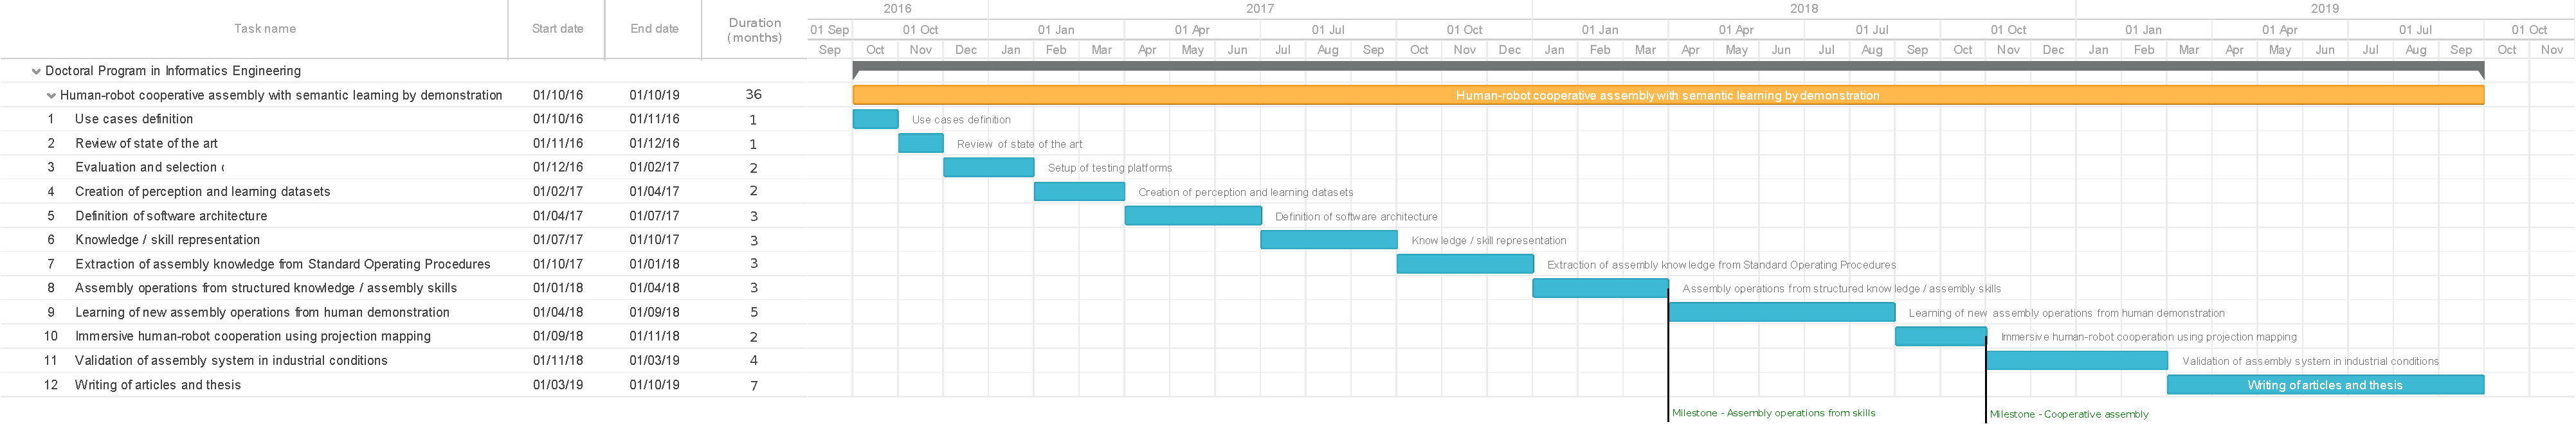
\includegraphics[trim={1.17cm 0 2.37cm 0},clip,height=.215\textheight,angle=90]{gantt-chart}
	\caption{Gantt chart with the main tasks and milestones}
	\label{fig:gantt-chart}
\end{figure}

